\documentclass[11pt,a4paper,oneside,german]{article}
\pagestyle{plain}
\usepackage[ngerman]{babel}
\usepackage[utf8]{inputenc}

\usepackage{geometry}
\geometry{a4paper,left=40mm,right=30mm, top=3.5cm, bottom=2.5cm}
\usepackage{graphicx}
\usepackage{hyperref}
\usepackage{float}
\usepackage{wrapfig}

\title{Praktikumsbericht Data Science 1}
\author{Robin Mayer, Nils Nover, Mariella Zunker}
\date{\today}

\begin{document}
	\maketitle
	
	\begin{figure}[h]
		\centering
		
\includegraphics[width=10.5cm]{uniemblem.jpg}		
	\end{figure}
	
	\newpage
	
	\tableofcontents
	
	\section{Fragestellung und Auswahl der Datensätze}
	
	Die Frage der Schädlichkeit von Stickoxiden und deren Zusammenhang mit Dieselfahrzeugen hat in der Vergangenheit die Debatte um die Verkehrswende dominiert. Um einen Überblick über die Rolle von verschiedenen Antriebsarten zu bekommen, sollten in diesem Projekt Daten zu Antriebsdaten mit Stickoxidwerten in Deutschland verglichen werden. \\
	Zu Analyse der Fragestellung wurden Datensätze des Umweltbundesamtes (UBA, 1) sowie des Kraftfahrtbundesamtes (KBA, 2) genutzt. Die Datensätze des UBA lagen als .xlx-Dateien vor und beinhalteten Informationen zu jahresgemittelten Stickoxidwerten an verschiedenen deutschen Messstationen(Abb. \ref{fig:BeispielNO2}), während das KBA hauptsächlich .pdf-Dateien veröffentlichte, in denen die zu einem Stichtag zugelassenen Anzahlen von Autos nach Antriebsart in den jeweiligen Orten aufgelistet waren (Abb. \ref{fig:BeispielKFZ}). Beide Quellen stellen Datensätze nach Jahr zu Verfügung.
	
	\begin{figure}[h!]
		\centering
		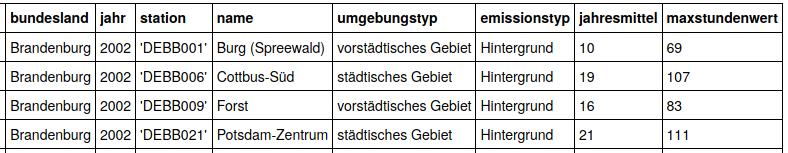
\includegraphics[width=10.5cm]{BeispielNO2.png}
		\caption{Auszug aus dem NO2-Datensatz.}
		\label{fig:BeispielNO2}
	\end{figure}
	
	\begin{figure}[h!]
		\centering
		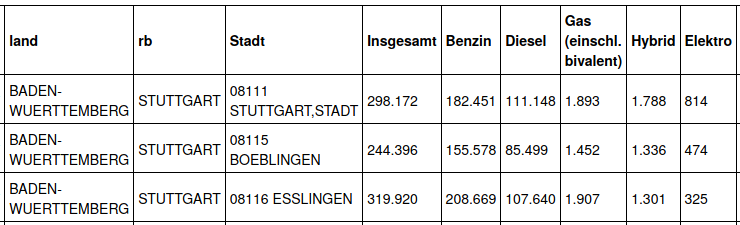
\includegraphics[width=10.5cm]{BeispielKFZ.png}
		\caption{Auszug aus dem KFZ-Datensatz.}
		\label{fig:BeispielKFZ}
	\end{figure}
	
	\section{Datenaufbereitung}
	
	Zunächst mussten die Datensätze in ein Format konvertiert werden, in dem sie sinnvoll verarbeitet werden konnten. Dazu wurden die .pdf-Dateien ins .xslx-Format konvertiert. Aufgrund der großen Unterschiede der beiden Formate musste hierbei jedoch manuell noch viel nachgebessert werden (WAS?), weshalb nicht alle zur Verfügung stehenden Jahrgänge ausgewertet werden konnten. Die .xlsx-Dateien konnten im Anschluss in ein .csv-Format konvertiert und als solches eingelesen werden.\\
	Aufgrund der guten Verfügbarkeit bestehender Tools und Libraries wurde für die Auswertung Python gewählt. Hierbei konnte vor allem auf das Datenanalysetool Pandas sowie Numpy und Matplotlib für die Auswertung zugegriffen werden. Das Jupyter Notebook stellt zudem eine übersichtliche und gut nachvollziehbare Programmierumgebung dar, in der Code gut im Team erarbeitet werden kann.\\
	Nach dem Einlesen wurden die Datensätze auf Vollständigkeit und Fehler durchsucht. Dabei wurde auf nicht erfasste Datenpunkte sowie offensichtliche Abweichungen wie negative Zahlen geachtet. Zudem mussten die Städtenamen und alle als String codierten Variablen überprüft und vereinheitlicht werden. So wurden alle Namen in Großbuchstaben und ohne Umlaute dargestellt, sowie Rechtschreibfehler und Unterschiede in der Darstellung von Doppelnamen korrigiert. Trennzeichen wie Komma oder Slash wurden vereinheitlicht und Zahlenwerte als Float gecastet. \\
	Zudem wurden Messwerte, die keinem eindeutigen Ort zugewiesen werden konnten (für einige Messwerte wurde als Bundesland "Umweltbundesamt" angegeben), aus dem Datensatz gelöscht, da eine nicht-automatisierte Zuordnung in der verfügbaren Zeit nicht möglich war. Schließlich wurde aus den einzelnen Dateien für jedes Jahr eine Gesamtdatei erstellt, in der alle Jahre enthalten waren. \\
	Insgesamt nahm die Aufbereitung der Daten viel Zeit in Anspruch. Mit mehr Kapazitäten hätten Fehlerbehebung und Vervollständigung der Daten noch stärker verfolgt werden können, indem beispielsweise alle Daten zugeordnet werden oder die Verteilung der Werte genauer betrachtet wird. In Abbildung \ref{fig:Heatmaps} sind beispielhaft einige Daten als Heatmaps dargestellt. Die weißen Bereiche stellen fehlende Daten dar.
	
	\begin{figure}[h!]
		\centering
		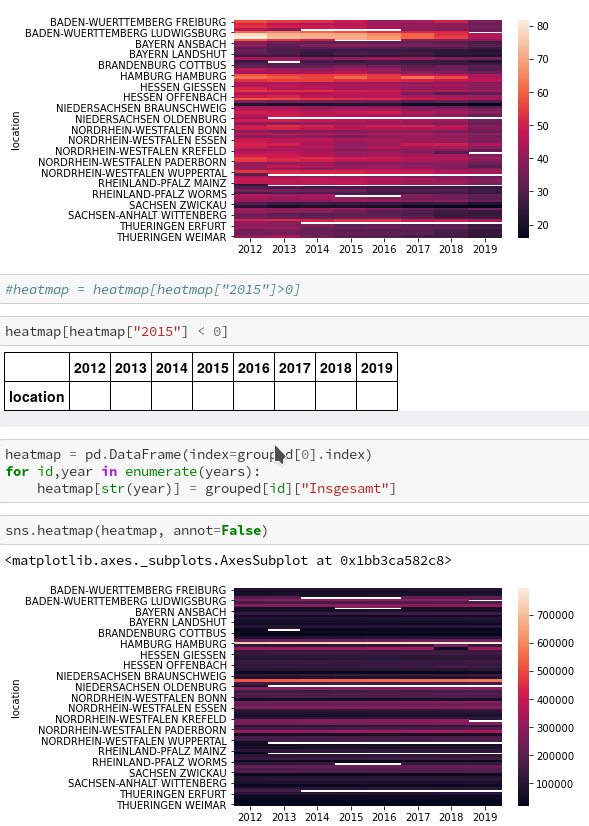
\includegraphics[width=12cm]{Heatmaps.png}
		\caption{Ausschnitt aus den Daten als Heatmaps dargestellt. Links die Stickstoffwerteentwicklung, rechts die Entwicklung der Autoanzahlen.}
		\label{fig:Heatmaps}
	\end{figure}
	
	\section{Datenauswertung}
	
	\subsection{Betrachtung der beiden Datensätze}
	
	Die Datensätze wurden zuerst isoliert betrachtet. Zur Messung der Luftwerte existierten Daten aus den Jahren 2002-2019, KfZ-Daten konnten von 2012-2019 genutzt werden. Die  Datensätze enthielten auch Zuordnungen der einzelnen Orte zu verschiedenen Abstufungen der Urbanität wie "vorstädtisches Gebiet". Die Einteilung wurde zur Vereinfachung zu den drei Kategorien "städtisch", "vorstädtisch" sowie "ländlich" zusammengefasst. Für einen ersten Überblick wurden die Stickoxidwerte über die Zeit geplottet (Abb. \ref{fig:NO2Entwicklung}). In der Tendenz stimmt das Ergebnis hierbei mit der Auswertung des Umweltbundesamtes (3) überein, die absoluten Werte weisen jedoch leichte Abweichungen auf. Dies ist wohl auf die leicht veränderte Einteilung der Orte in die drei Kategorien zurückzuführen.\\
	
	\begin{figure}[h!]
		\centering
		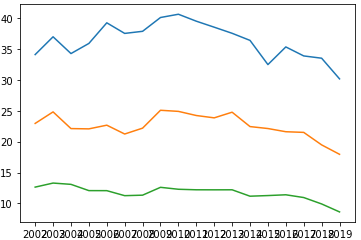
\includegraphics[width=8.5cm]{NO2Entwicklung.png}
		\caption{Entwicklung der Stickoxide über die Zeit. Blau: Städtisch. Gelb: Vorstädtisch. Grün: Ländlich.}
		\label{fig:NO2Entwicklung}
	\end{figure}
	
	Zur weiteren Analyse wurden die Datensätze im Anschluss zusammengefügt. Dabei sollten die Stickstoffdaten den Kraftfahrzeugdaten über die Orte zugeordnet werden. Um Verwechslungen bei gleichem Namen zu vermeiden, wurde dazu pro Jahr und Bundesland überprüft, ob eine Stadt im Stickstoff-Datensatz auch im KfZ-Datensatz existiert und bei Übereinstimmung wurden die Daten in neuen Spalten hinzugefügt. Dieses Merging stellte eine größere Herausforderung dar als vermutet, da die Datensätze nicht die gleiche Zuordnung der Werte zu den Orten enthielten wie zunächst angenommen. So bezogen sich die Daten des Kraftfahrtbundesamtes auf die regulären Landkreise, die Messungen des UBA waren jedoch lediglich dem nächsten Ort zugewiesen und nicht der offiziellen Kreisstadt. Diese Zuordnung führte dazu, dass beim Merging ländliche Gebiete weniger gut zugeordnet werden konnten als größere Städte (Abb. \ref{fig:Kategorien}).\\
	
	\begin{wrapfigure}{r}{0.4\textwidth}
		\vspace{-20pt}
		\begin{center}
			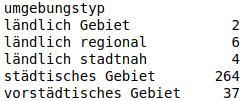
\includegraphics[width=4.5cm]{Kategorien.jpg}
			\caption{Anzahl an Orten in den Kategorien, die zugeordnet werden konnten, beispielhaft am Jahr 2017.}
			\label{fig:Kategorien}
		\end{center}
		\vspace{-20pt}
	\end{wrapfigure}
	
	Zudem ist zu beachten, dass einige Städte in den Datensätzen mehrfach vorkommen (z.B. Weimar Schwanseestr. und Weimar Steubenstr.). Um hier einer Stadt mehrere Messstationen zuordnen zu können wurde zur Vereinfachung der Mittelwert dieser Stationen verwendet. Das Merging beanspruchte einen Großteil der Zeit des gesamten Projektes und konnte dennoch nicht die angestrebte Vollständigkeit erreichen. Wäre mehr Zeit vorhanden, hätten noch mehr Versuche angestrengt werden können, alle Städte in den beiden Datensätzen zuzuordnen. Möglich wäre dabei, die Orte eindeutig mithilfe eines Karten-Tools zu ermitteln und zuzuordnen. Auch auf Ausreißer hätte mehr geachtet werden können. Zudem wäre es noch interessant gewesen, die zeitliche Entwicklung in den Daten zu betrachten und diese in gesellschaftliche Kontexte zu setzen, wie zum Beispiel Gesetzesänderungen, Umweltzonen und lokale Unterschiede. (Outlook hier oder in der Diskussion?)
	
	\subsection{Betrachtung der Werte und lineare Regression}
	
	Im Anschluss an die Zuordnung wurden die Stickstoffwerte gegen die Fahrzeugzahlen aufgetragen. Dabei konnte bereits ein grober Trend erkannt werden. Mithilfe linearer Regression wurde versucht, den Zusammenhang genauer zu beschreiben (\ref{fig:linreginsgesamt}). Außerdem zeigten sich im Bereich der Fahrzeugzahlen einige extreme Ausreißer
	
	\begin{figure}[h!]
		\centering
		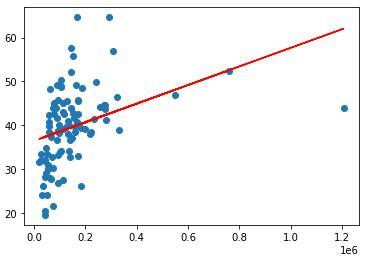
\includegraphics[width=6.5cm]{linreginsgesamt.jpg}
		\caption{Stickstoffwerte in Abhängigkeit der Fahrzeugzahlen.}
		\label{fig:linreginsgesamt}
	\end{figure}
	
	Das Ergebnis wurde anschließend mithilfe von drei Error-Parametern evaluiert. Dabei zeigte sich ein mittlerer absoluter Fehler von 6,21, ein MSE von 66,82 sowie ein R2-Score von 0,13. Die gefundene Regressionsgerade beschreibt den gefundenen Zusammenhang somit eher weniger gut. \\
	Die Auswertung wurde schließlich noch einmal unter Ausschluss der Ausreißer durch-geführt, brachte jedoch keine nennenswerte Besserung. \\
	Als nächstes wurde der Anteil an Dieselfahrzeugen betrachtet und die Stickstoffwerte gegen diesen aufgetragen. Eine grobe Betrachtung des Plots ließ zunächst auf eine eher zufällige Verteilung mit geringfügiger linearer Tendenz schließen. Auch durch lineare Regression konnte hierbei kein starker Zusammenhang festgestellt werden (Abb. \ref{fig:linregdieselanteil}).
	
	\begin{figure}[H]
		\centering
		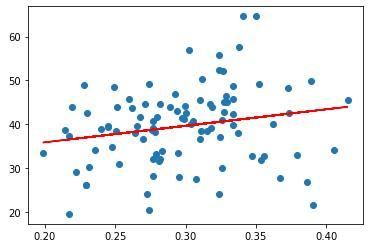
\includegraphics[width=6.5cm]{linregdieselanteil.jpg}
		\caption{Stickstoffwerte in Abhängigkeit des Dieselanteils.}
		\label{fig:linregdieselanteil}
	\end{figure}
	
	Die Evaluation ergab hierbei einen absoluten durchschnittlichen Fehler von 6,64, einen MSE von 74,04 sowie einen R2-Score von 0,04, und lässt darauf schließen, dass hier kein sinnvoller Erkenntnisgewinn durch die lineare Regression geschaffen wurde.
	
	\subsection{Nicht-lineare Regression}
	
	Rund 38\% der Bundesweiten NOx Belastung stammt laut UBA aus dem Verkehr (3). Die betrachteten Messstationen tragen die Bezeichnung "Verkehr". Da es sich außerdem meist um Großstädte handelt, steuern andere NO2 Quellen, wie Land und Energiewirtschaft, einen untergeordneten Beitrag zur NO2 Bilanz bei. Der lineare Zusammenhang scheint also zunächst naheliegend. Je mehr PKWs in einer Stadt zugelassen sind, desto mehr NO2 Belastung könnte entstehen. Hier werden allerdings einige Aspekte nicht beachtet. Die Größe des Stadtgebietes und physikalische Eigenschaften der Gase wie Diffusion könnten dafür sorgen, dass sich der Zusammenhang mit einer Wachstumskurve womöglich genauer beschreiben lässt. Die Auslastung der Straßen, an denen der NO2 Wert gemessen wird, ist je nach Größe auf einen bestimmten Verkehrsdurchfluss begrenzt. Neue Fahrzeuge in der Stadt sorgen hier also nicht gleichzeitig für einen hören NO2 Wert. Daher ist es möglich, dass eine Sättigungskurve die NO2-Entwicklung besser beschreibt. Es wurde also noch eine nicht-lineare Regressionsanalyse durchgeführt (Abb. \ref{fig:nonlinreg}).
	
	\begin{figure}[H]
	\centering
	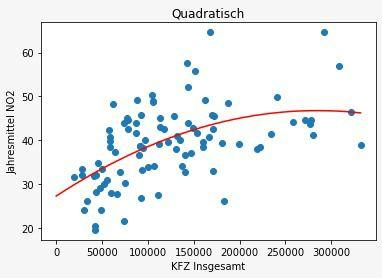
\includegraphics[width=6.5cm]{nonlinreg.jpg}
	\caption{Nicht-lineare Regression des Zusammenhangs von Fahrzeugzahlen und Stickstoffwerten.}
	\label{fig:nonlinreg}
	\end{figure}
	
	\section{Diskussion}
	
	Ziel der Analyse war es, den Zusammenhang zwischen Stickstoffwerten und Anzahl an Fahrzeugen einerseits sowie Dieselfahrzeugen andererseits zu untersuchen. Der erste Punkt konnte durch die Daten zwar recht gut gezeigt werden, doch die Regressionsanalyse zeigt, dass zusätzliche Daten benötigt werden, um den Zusammenhang genau zu beschreiben. So stellt sich beispielsweise die Frage, ob die Autos dort, wo sie gemeldet sind, auch tatsächlich gefahren werden. So stellen beispielsweise Mietwagenfirmen, die ihre Fahrzeuge alle in einer Stadt melden, ein Problem bei der hier dargestellten Vorgehensweise dar. Es wäre also besser, Fahrzeugdaten zu verwenden, die klar an einer Stelle nachgewiesen wurden. (was meinen wir hier? Ich meine abgesehen von gewerblich genutzten Fahrzeugen würde ich schon sagen dass im Durchschnitt überall in Deutschland zu ähnlichen Prozentsätzen dort gefahren wird, wo auch zugelassen wurde. Klar gibt es hier viel Rauschen aber im großen und ganzen finde ich unseren approach nich bad) \\
	Bei der Analyse der Dieselfahrzeuge konnte kein zuverlässiger Zusammenhang gefunden werden. Allerdings sind auch bei der Interpretation dieser Ergebnisse einige Punkte zu beachten. Die Einteilung in Diesel/Nicht-Diesel kann hierbei als zu grob betrachtet werden. \\
	Insgesamt war vor allem die Datenaufbereitung und die Zuordnung der Datensätze zueinander mit Schwierigkeiten verbunden. Mit etwas mehr Zeit wäre es vielleicht möglich gewesen, alle älteren Jahrgänge der KBA in die Analyse aufzunehmen und sich die zeitliche Entwicklung noch genauer anzusehen. Die Ergebnisse zeigten zwar leicht sinkende Stickstoffwerte über die Zeit, doch von genauerem Interesse wären auch noch lokale Unterschiede wie Umweltzonen oder Ballungsräume. \\
	Auch der Vergleich von urbanen und ländlichen Gebieten konnte aufgrund der Herausforderungen bei der Fusion der Datensätze nicht gezogen werden. Wenn die Städte eindeutiger zuzuordnen wären, wäre hier noch eine genauere Analyse von Einflussfaktoren möglich gewesen. \\
	
	\section{Quellen}
	
	(1) https://www.umweltbundesamt.de/themen/luft/luftschadstoffe/stickstoffoxide\\
	(2) https://www.kba.de/DE/Statistik/Fahrzeuge/Bestand/ZulassungsbezirkeGemei-nden/zulassungsbezirke\_node.html\\
	(3) https://www.umweltbundesamt.de/themen/luft/daten-karten/entwicklung-der-luftqualitaet\#entwicklung-der-luftqualitat-in-deutschland \\
	
	
	
\end{document}